\documentclass[a4paper, 12pt]{article}

\usepackage[T2A]{fontenc}
\usepackage[utf8]{inputenc}
\usepackage[english,russian]{babel}
\usepackage[left=15mm, top=20mm, right=15mm, bottom=20mm, nohead, nofoot]{geometry}

\usepackage{hyperref}
\usepackage{graphicx}
\usepackage{wrapfig}
\usepackage{afterpage}
\usepackage{amsmath, amsfonts, amssymb, amsthm, mathtools}
\author{Хомутов Андрей, группа Б06-903}
\title{ВПВ по курсу "Электричество и магнетизм" \\ Конденсатор на высоких частотах}
\date{22 декабря 2020 г.}
%%%%%%%%%%%%%%%%%%%%%%%%%%%%%%%%%%%%%%%%%%%%%%%%%%%%%%%%%%%%%%%%%%%%%%%%%
\usepackage{graphicx, wrapfig, subcaption, setspace, booktabs}
\usepackage[protrusion=true, expansion=true]{microtype}
\usepackage[english]{babel}
\usepackage{sectsty}
\usepackage{url, lipsum}
\newcommand{\HRule}[1]{\rule{\linewidth}{#1}}
\onehalfspacing
\setcounter{tocdepth}{5}
\setcounter{secnumdepth}{5}
%%%%%%%%%%%%%%%%%%%%%%%%%%%%%%%%%%%%%%%%%%%%%%%%%%%%%%%%%%%%%%%%%%%%%%%%%


\begin{document}

\title{ \normalsize \textsc{Лабораторная работа по общей физике}
		\\ [4.0cm]
		\HRule{0.5pt} \\ [0.3cm]
		\LARGE \textbf{{Изучение спектров атома $H$ и молекулы $I_2$}}
		\HRule{0.5pt} \\ [0.1cm]
		\normalsize  \vspace*{18\baselineskip}}

\date{}

\author{
		Хомутов Андрей, Б06-903 \\
		Рыбкина Елизавета, Б06-903\\
ФБМФ, 2021\\ }

\maketitle
\thispagestyle{empty}
\newpage
%%%%%%%%%%%%%%%%%%%%%%%%%%%%%%%%%%%%%%%%%%%%%%%%%%%%%%%%%%%%%%%%%%%%%%%%%

%%%%%%%%%%%%%%%%%%%%%%%%%%%%%%%%%%%%%%%%%%%%%%%%%%%%%%%%%%%%%%%%%%%%%%%%%
 
\section{Теоретическая часть}
Атом водорода является простейшей атомной системой; для него уравнение Шредингера можно решить точно. 

Длины волн спектральных линий описываются формулой 
\begin{equation}
\dfrac{1}{\lambda_{mn}} = RZ^2\left(\frac{1}{n^2} - \frac{1}{m^2}\right),
\end{equation}
где $R$ --- постоянная Ридберга, а $m$ и $n$ --- целые числа.

Для объяснения спектра атома водорода Нильс Бор в 1913 г. предложил теория атома, основанную на трех постулатах:

\begin{enumerate}
\item Из всех возможных с точки зрения классической физики орбит в атоме осуществляются только некоторые стационарные орбиты,при движении по которым, вопреки представлениям классической электродинамики, электрон не излучает энергии;
\item Из всех возможных орбит в атоме осуществляются только те, для которых момент количества движения равен целому кратному величины постоянной Планка $\hbar = h/(2\pi)$ т.е.
\begin{equation}
L = n \hbar
\end{equation}
\item Излучение или поглощение энергии происходит при переходе атома из одного стационарного состояния в другое, а частота излучаемого света связана с разностью энергий атома в стационарных состояниях соотношением 
\begin{equation}
h \nu = E_2 - E_1,
\end{equation}
где $\nu$ --- частота излучаемой линии.
\end{enumerate}

Использование этих постулатов с учетом кулоновского взаимодействия между ядром и электроном позволяет определить энергетические уровни:
\begin{equation}
E_n = - \frac{2\pi^2m_ee^4Z^2}{h^2}\frac{1}{n^2}
\end{equation}

А из формулы $(4)$ можно определить возможные частоты излучения. 

Из рис. 1 видно, что линии в спектре водорода можно расположить по сериям; для всех линий $n$ постоянно, а $m$ меняется от $n+1$ до $\infty$. 

В данной работе изучается серия Бальмера, линии которой лежат в видимой области. 

\begin{figure}[h]
    \centering
    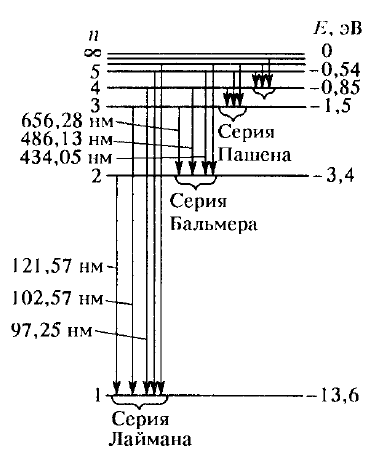
\includegraphics[width=6cm]{fig3.PNG}
    \caption{Уровни энергии атома водорода и образование спектральных серий}
    \label{fig:vac}
\end{figure}

Для серии Бальмера $n=2$, а $m = 3, 4, 5, 6$. Эти линии обозначаются $H_{\alpha}, H_{\beta}, H_{\gamma}, H_{\delta}$.

Энергия основного состояния выражается как:
\begin{equation}
E = -RZ^2
\end{equation}

Аналогично энергия возбужденных состояний:
\begin{equation}
E_n = -R\frac{Z^2}{n^2}
\end{equation}

\newpage
\section{Практическая часть}
\subsection{Калибровка и снятие спектров водорода и йода}
По спектрам неона и ртути была построена калибровочная кривая (синяя линия на рис.2). Аппроксимация проводилась полиномом 3й степени $y = a_0 + a_1x + a_2x^2 + a_3x^3$, где $a_0 = 3780\pm30$, $a_1 = 0,93\pm0,09$, $a_2 = (-4,7\pm0,6) \cdot 10^{-4}$, $a_3= (2,2 \pm 0,14) \cdot 10^{-7}$. 

Длины волн линий равны соответственно $H_{\alpha} = 6548$, $H_{\beta} = 4846$, $H_{\gamma} = 4362$, $H_{\delta} = 4110$ ангстрем, что достаточно близко к справочным значениям с учетом значительной погрешности, превышающей как минимум 30 А для данной аппроксимации. Отношение длин волн практически соответствует ожидаемому из формулы (1) - $1:1,351:1,501:1,593 \simeq 1:1,35:1,512:1,6$.

Также по формуле (1) можно посчитать постоянную Ридберга для каждой линии, а затем усреднив $R \simeq 109665	\pm 340$ обратных сантиметров, что крайне близко к справочному $R_0 = 109677,6$.

\begin{figure}[h!]
    \begin{center}
    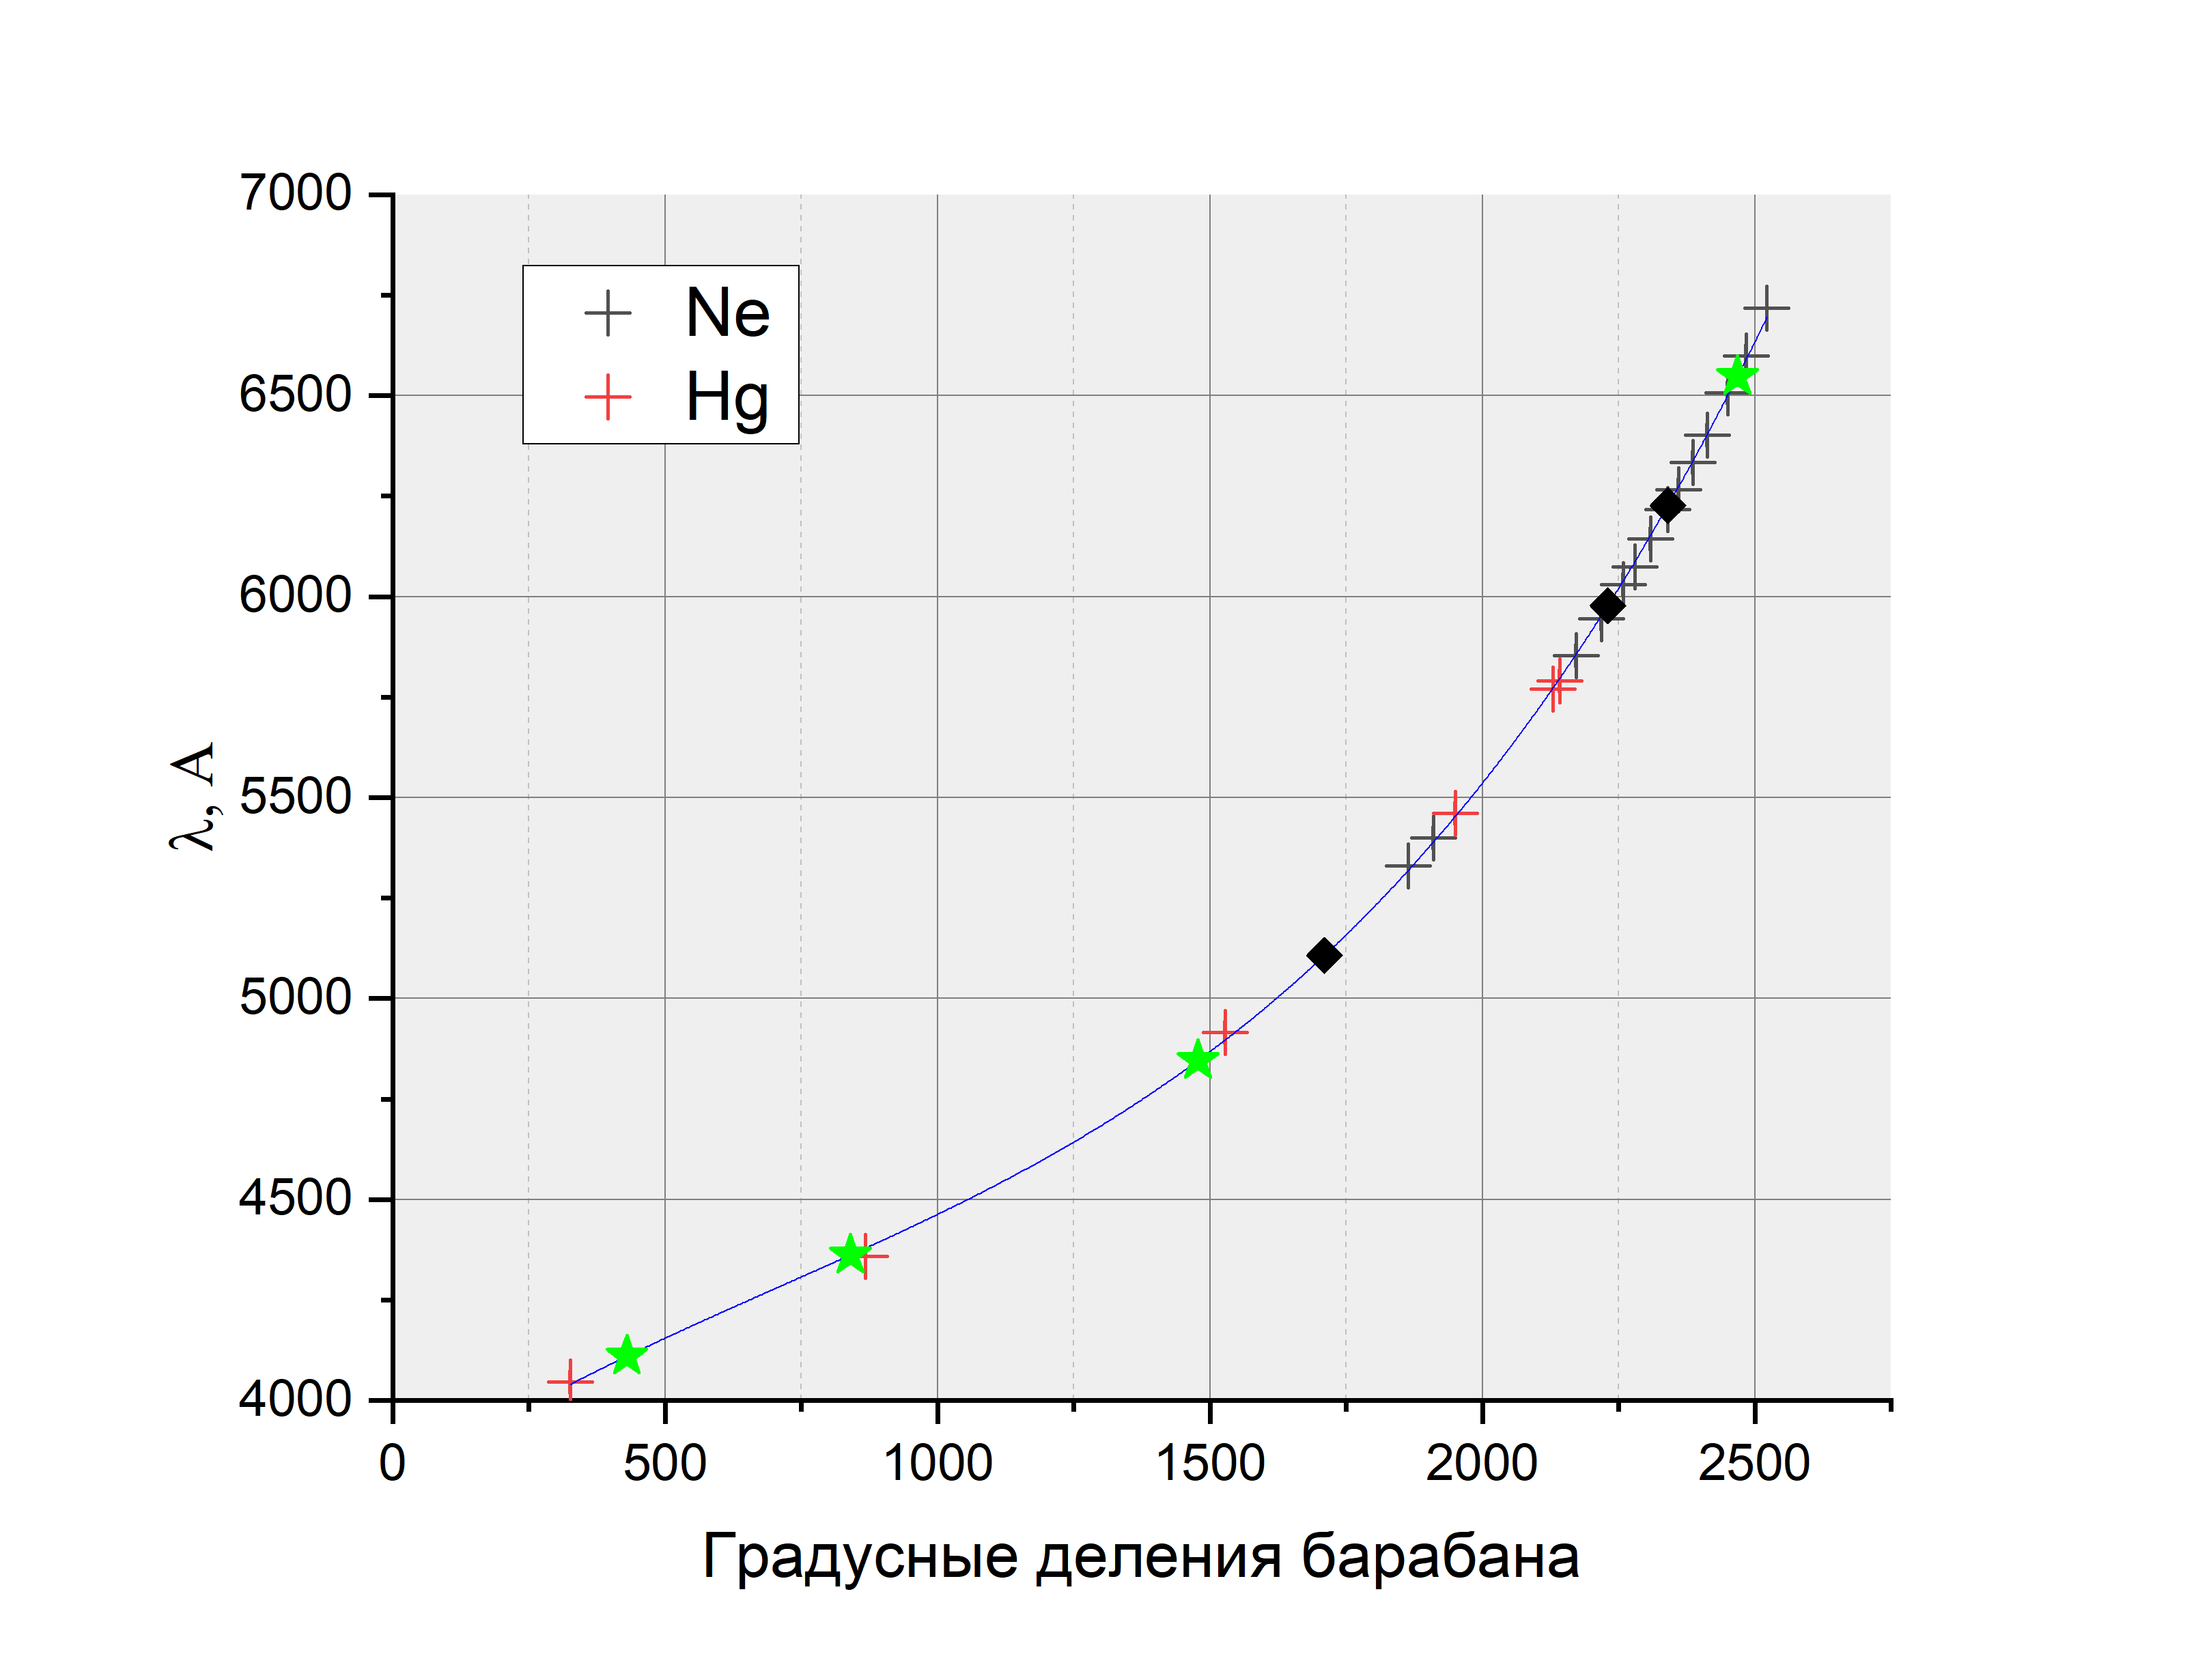
\includegraphics[width=0.8\textwidth]{calibrovka.png}
    \end{center}
    \caption{График калибровки и линий водорода и йода}
\end{figure}

Для йода также можно определить $h\nu_{1,0} = 1,99 \pm 0,13, h\nu_{1,5}=2,07 \pm 0,27, h\nu_{\text{гр}}=2,4 \pm 0,3$ эВ.

Вычислим также энергию колебательного кванта возбужденного состояния молекулы йода:
\[h\nu_2 = (h\nu_{1,5}-h\nu_{1,0})/5 \simeq 0,0165\]

Также известно что для основного состояния $h\nu_1 = 0,027$ эВ, a энергия возбуждения атома равна $E_A = 0,94$ эВ. Учитывая что $h\nu_{\text{гр}} = h\nu_e + D_2 = D_1 + E_a$ и $h\nu_{0,n_2} = h\nu_e + h\nu_2\left(n_2 + \frac{1}{2}\right) - \frac{1}{2}h\nu_1$, $h\nu_e = 1,96 \pm 0,14, D_1=1,49 \pm 0,3, D_2 \simeq 0,47$ эВ.


\end{document}

%%%%%%%%%%%%%%%%%%%%%%%%%%%%%%%%%%%%%%%%%%%%%%%%%%%%%%%%%%%%%%%%%%%%%%%%%
 \section{Выводы}
\begin{enumerate}
    \item По полученным значениям длин волн была вычислена постоянная Ридберга с ошибкой в пятом (!) знаке, хотя 
    \item 

\end{enumerate}

\end{document}

\begin{table}[h!]
\begin{center}
\caption{...}
\begin{tabular}{|c|c|c|c|c|}

\end{tabular}
\end{center}
\end{table}


\begin{figure}[h!]
    \begin{center}
    \includegraphics[width=0.8\textwidth]{xxx.png}
    \end{center}
    \caption{...}
\end{figure}

\begin{figure}[h!] %% ШАБЛОН ДЛЯ ДВУХ КАРТИНОК
\begin{center}
\begin{minipage}[h]{0.40\linewidth}
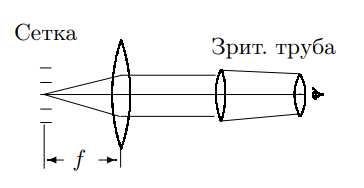
\includegraphics[width=1\linewidth]{plus_lens.PNG}
\caption{...} %% подпись к рисунку
\label{ris:experimoriginal} %% метка рисунка для ссылки на него
\end{minipage}
\hfill 
\begin{minipage}[h]{0.40\linewidth}
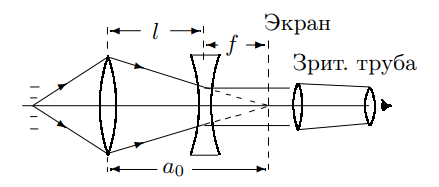
\includegraphics[width=1\linewidth]{minus_lens.PNG}
\caption{..}
\label{ris:experimcoded}
\end{minipage}
\end{center}
\end{figure}

\subsection{...}
\subsubsection{...}



\subsubsection{...}